\clearpage
\section*{Section A (Numerical Oscillations of Discretization Rules)}
\addcontentsline{toc}{section}{Section A (Numerical Oscillations of Discretization Rules)}

One way to analyze the properties of various discretization methods (e.g., in terms of their numerical oscillations) is to solve a lossless first-order system (e.g., inductance or capacitance) when the state variable of the component is suddenly changed. The circuit on the right considers a case where a dc voltage is suddenly applied to a capacitor. Because the source voltage is applied like a step function, we know that the current of the capacitor should look like an impulse, analytically. Let us assume that in the simulations all the variables are zero at $t=0$ and the voltage source takes its value at $t=\Delta t$.

\begin{figure}[h!]
    \centering
    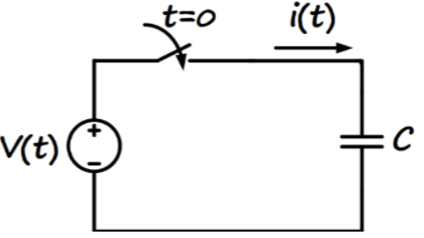
\includegraphics[width=0.4\textwidth]{figures/figure-A-circuit.png}
    \caption{Simple capacitor circuit with DC voltage source}
    \label{fig:a01_circuit}
\end{figure}

1) Determine the step-by-step solution for the current in the capacitor (in terms of capacitance $C$, time-step size $\Delta t$, and source voltage) using the following discretization rules: a) Forward Euler, b) Backward Euler, c) Trapezoidal.

\vspace{1em}
% Your solution here
